%Capítulo 1 - Introducción
\chapter{Introducción}
\label{chap:1}

\section{Motivación y objetivo general}
\label{sec:mot}

\begin{figure}[H]
    \centering
    \subbottom[\label{sfig:mot.1}]{\scalebox{.9}{\begin{tikzpicture}

  \node[tplace] (p0) at (-.5,0) {};
  \node[tplace] (p0') at (.5,0) {};
  \node[transition] (x) at (0,-1) {$a$};
  \node[tplace] (p1) at (0,-2) {};
  \node[transition] (y) at (0,-3) {$b$};
  \node[tplace] (p3) at (1.25,-1) {};
  \node[transition] (z) at (1.25,-2) {$c$};
  \node[tplace] (p4) at (1.25,-3) {};
  \node[tplace] (p5) at (-1,-3) {};
        
  \node[] (t) at (p0) {6};
  \node[] (t) at (p0') {1};
  \node[] (t) at (p3) {2};
  \node[] (t) at (p5) {3};
      
  \draw[style={->,>=triangle 45}] (p0) edge node[right,yshift=1.25mm,xshift=-.75mm]{\scriptsize 3} (x);
  \draw[style={->,>=triangle 45}] (p0') to (x);
  \draw[style={->,>=triangle 45}] (x) to (p1);    
  \draw[style={->,>=triangle 45}] (p1) to (y);      
  \draw[style={->,>=triangle 45},bend left=30] (y) edge node[left]{\scriptsize 2} (p0);
  \draw[style={->,>=triangle 45},bend right=30] (y) to (p0');
  
  \draw[style={->,>=triangle 45}] (p3) to (z);      
  \draw[style={->,>=triangle 45}] (p1) to (z);      
  \draw[style={->,>=triangle 45}] (z) to (p4);

  \draw[style={->,>=triangle 45}] (p5) to (y);

%\node[] (name) at (.5,-4) {$N_1$};
  
\end{tikzpicture}
}}
    \hspace{10mm}
    \subbottom[\label{sfig:mot.2}]{\scalebox{.9}{\begin{tikzpicture}

  \node[tplace] (p0) at (-.5,0) {};
  \node[tplace] (p0') at (.5,0) {};
  \node[transition] (x) at (0,-1) {$a$};
  \node[tplace] (p1) at (0,-2) {};
  \node[transition] (y) at (0,-3) {$b$};
  \node[tplace] (p3) at (1.25,-1) {};
  \node[transition] (z) at (1.25,-2) {$c$};
  \node[tplace] (p4) at (1.25,-3) {};
  \node[tplace] (p5) at (-1,-3) {};
        
  \node[] (t) at (p0) {2};
  \node[] (t) at (p0') {1};
  \node[] (t) at (p3) {2};
  \node[] (t) at (p5) {3};
    
  \draw[style={->,>=triangle 45}] (p0) to (x);
  \draw[style={->,>=triangle 45}] (p0') to (x);
  \draw[style={->,>=triangle 45}] (x) to (p1);    
%  \draw[style={->,>=triangle 45}] (p1) to (z);      
  \draw[style={->,>=triangle 45}] (p1) to (y);      
  \draw[style={->,>=triangle 45},bend left=30] (y) to (p0);
  \draw[style={->,>=triangle 45},bend right=30] (y) to (p0');

  \draw[style={->,>=triangle 45}] (p3) to (z);      
  \draw[style={->,>=triangle 45}] (z) to (p4);

  \draw[style={->,>=triangle 45}] (p5) to (y);


  %\node[] (name) at (.5,-4) {$N_2$};

\end{tikzpicture}
}}
    \hspace{10mm}
    \subbottom[\label{sfig:mot.3}]{\scalebox{.9}{\begin{tikzpicture}

  \node[tplace] (p0) at (-.5,0) {};
  \node[tplace] (p0') at (.5,0) {};
  \node[transition] (x) at (0,-1) {$a$};
  \node[tplace] (p1) at (0,-2) {};
  \node[transition] (y) at (0,-3) {$b$};
  \node[tplace] (p3) at (1.25,-1) {};
  \node[transition] (z) at (1.25,-2) {$c$};
  \node[tplace] (p4) at (1.25,-3) {};
  \node[tplace] (p5) at (-1,-3) {};
        
  \node[] (t) at (p0) {2};
  \node[] (t) at (p0') {1};
  \node[] (t) at (p3) {2};
  \node[] (t) at (p5) {3};
    
  \draw[style={->,>=triangle 45}] (p0) to (x);
  \draw[style={->,>=triangle 45}] (p0') to (x);
  \draw[style={->,>=triangle 45}] (x) to (p1);    
  \draw[style={->,>=triangle 45}] (p1) to (z);      
  \draw[style={->,>=triangle 45}] (p1) to (y);      
  \draw[style={->,>=triangle 45},bend left=30] (y) to (p0);
  \draw[style={->,>=triangle 45},bend right=30] (y) to (p0');

  \draw[style={->,>=triangle 45}] (p3) to (z);      
  \draw[style={->,>=triangle 45}] (z) to (p4);

  \draw[style={->,>=triangle 45}] (p5) to (y);


  %\node[] (name) at (.5,-4) {$N_3$};

\end{tikzpicture}
}}
    \hspace{10mm}
    \subbottom[\label{sfig:mot.4}]{\scalebox{.9}{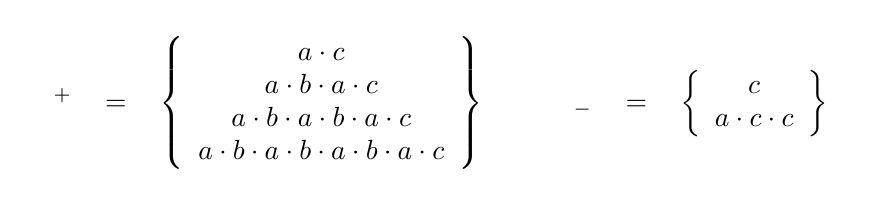
\begin{tikzpicture}

\node[] (logs) at (0,0) {

\begin{tabular}{rcl}
  $\pmlog^+$ & = &
  $\left \{
  \begin{array}{c}
  a \cdot c \\
  a \cdot b \cdot a \cdot c \\
  a \cdot b \cdot a \cdot b \cdot a \cdot c \\
  a \cdot b \cdot a \cdot b \cdot a \cdot b \cdot a \cdot c \\
  \end{array}
  \right \}$
\end{tabular}  
\hspace{5mm}
\begin{tabular}{rcl}
  $\pmlog_-$ & = &
  $\left \{
  \begin{array}{c}
  c \\
  a \cdot c \cdot c
  \end{array}
  \right \}$
\end{tabular}
};

%\node[] (null) at (0,-2) {};

\end{tikzpicture}}}
    \caption{Tres modelos de procesos que ilustran el descubrimiento supervisado de procesos}
    \label{fig:mot}
\end{figure}


\section{Estado del arte}
\label{sec:antecedentes}
El arte es morirte de frío. Solo que no morirte, otra cosa.

\section{Alcance del trabajo}
\label{sec:alcance}
Hasta la esquina, después me canso

\section{Estructura de la tesina}
\label{sec:estructura}
Primero viene el~\autoref{chap:1},
después el~\autoref{chap:2},
después el~\autoref{chap:3},
después el~\autoref{chap:4}
y por último el~\autoref{chap:5}
